\chapter{Validazione della soluzione}\label{chap:Validazione della soluzione}
Per procedere alla validazione della soluzione proposta, è stato preparato un ambiente Kubernetes in esecuzione su Minikube, che a sua volta è in esecuzione su un container Docker\footnote{https://www.docker.com}. Sebbene questo ambiente sia notoriamente più piccolo rispetto ai dispiegamenti tipici su microservizi, rimane un valido strumento per il testing della soluzione proposta, trattandosi a tutti gli effetti di un ambiente Kubernetes.

Tutti i log delle validazioni della soluzione sono disponibili nella repository del progetto, trattata al Capitolo \ref{chap:Realizzazione della soluzione}. In particolare, nella cartella \textit{output\_logs}, è presente una cartella per ogni test della soluzione proposta. La struttura dei file segue lo schema descritto di seguito:
\begin{itemize}
    \item \textit{all.log}: contiene i log di tutte le interazioni scambiate tra i microservizi.
    \item \textit{event.log}: contiene l'evento di interesse che si vuole ispezionare tramite yRCA.
\end{itemize}
\section{Iniezione di un fallimento nell'applicazione Bookinfo} \label{sect:Iniezione di un fallimento nell'applicazione Bookinfo}
\subsection{Introduzione a Bookinfo}
Istio, come la maggior parte delle piattaforme moderne, fornisce un'applicazione di esempio per aiutare gli sviluppatori a familiarizzare con le sue funzionalità. L'applicazione di esempio offerta da Istio è chiamata \myenquote{Bookinfo}\footnote{https://istio.io/latest/docs/examples/bookinfo/}. Questo capitolo fornisce una panoramica dell'applicazione Bookinfo, e come è stata usata a scopi di test per testare il funzionamento della soluzione.

Bookinfo è un'applicazione a microservizi che mostra informazioni sui libri in una sorta di negozio online. Composta da molteplici componenti, ognuno di essi si trova in un deployment separato:
\begin{itemize}
    \item \textit{Productpage:} Microservizio contenente un server Web che rende possibile la visualizzazione di una semplice pagina Web. Internamente, è anche responsabile di chiamare i servizi interni .
    \item \textit{Details:} Microservizio contenente le informazioni dettagliate dei libri.
    \item \textit{Reviews:} Microservizio utilizzato per mostrare le recensioni degli utenti. È presente in tre versioni:
    \begin{itemize}
        \item \textit{v1:} Versione che non mostra recensioni degli utenti.
        \item \textit{v2:} Versione che mostra recensioni degli utenti, con stelle nere.
        \item \textit{v3:} Versione che mostra recensioni degli utenti, con stelle rosse.
    \end{itemize}
    \item \textit{Ratings:} Microservizio chiamato dalla versione v2 e v3 di \textit{Reviews}, e produce una valutazione per un libro.
\end{itemize}

La Figura \ref{fig:with_istio} mostra il suddetto ambiente.

\begin{figure}[h]
    \centering
    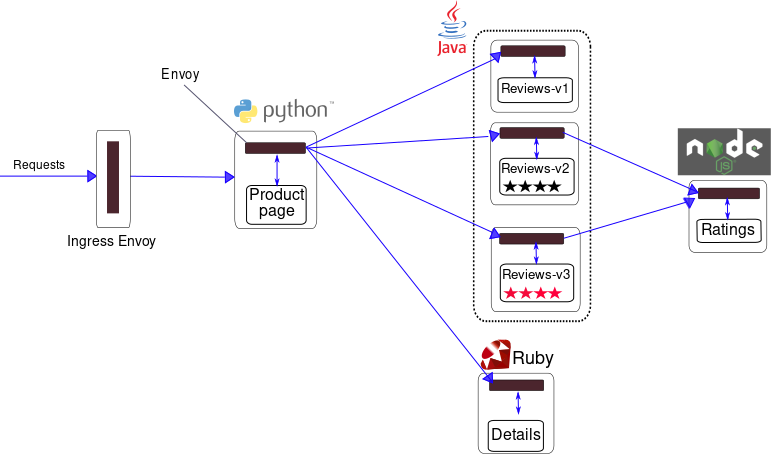
\includegraphics[width=\textwidth]{immagini/capitolo5/withistio.png}
    \caption{Schema fornito da Istio per Bookinfo \cite{istio_bookinfo}.}
    \label{fig:with_istio}
\end{figure}

Il microservizio su cui si vuole generare un fallimento per questa dimostrazione è \texttt{Ratings}, in quanto trattasi di un servizio cruciale e non ridondante.


Il metodo che sarà usato per interrompere il traffico tra \texttt{Reviews} e \texttt{Ratings} sarà quello di simulare un blocco interno al container \texttt{Ratings}, come in Figura \ref{fig:with_istio_broken}.

\begin{figure}[h]
    \centering
    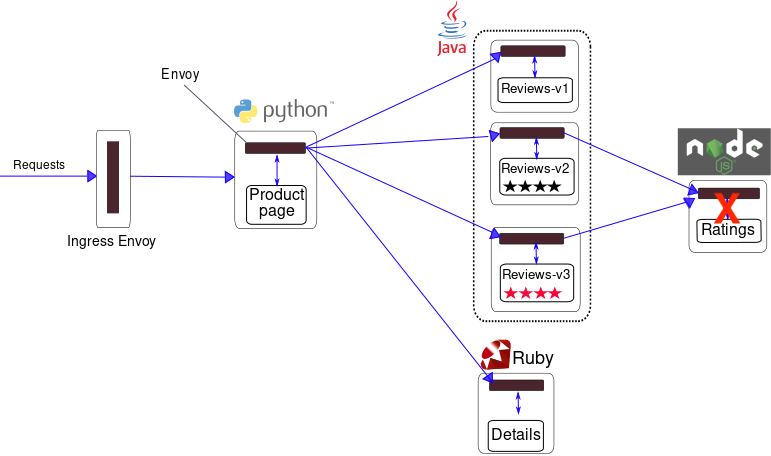
\includegraphics[width=\textwidth]{immagini/capitolo5/withistio_broken.png}
    \caption{Punto di simulazione del fallimento.}
    \label{fig:with_istio_broken}
\end{figure}


Per fare ciò, saranno usate delle funzionalità di Docker e Minikube che consentono di interrompere l'elaborazione di un container senza spegnerlo completamente. La differenza, infatti, sta nel modo in cui viene gestito questo fallimento da Kubernetes: simulando un crash del container il processo non sarebbe dimostrabile, perché Kubernetes tenta sempre di riavviare il pod o container interrotto.
\subsection{Iniezione del fallimento}\label{Iniezione del fallimento}
Per prima cosa, viene eseguito il tool Python che trasforma il deployment originale di Bookinfo in un deployment con le funzionalità di logging descritte nei capitoli precedenti. Dopo di esso, si applicano al cluster le CRD, e il deployment modificato al cluster, tramite l'esecuzione dei comandi descritti nel Codice \ref{lst:code_run_script}:

\begin{lstlisting}[caption={Comandi per l'applicazione dei CRD e del deployment modificato.}, label=lst:code_run_script, language=bash]
python main.py -i <file_input> -o <file_output>
kubectl apply -f crds.yaml
kubectl apply -f <file_output.yaml>
\end{lstlisting}
\begin{figure}[H]
    \centering
    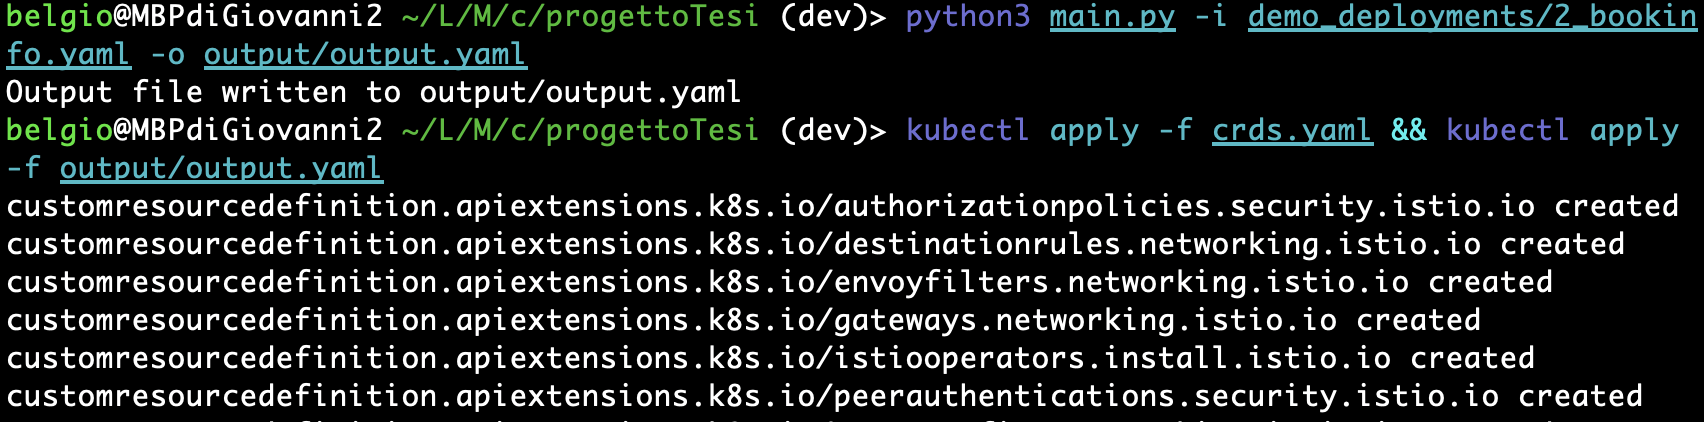
\includegraphics[width=\textwidth]{immagini/capitolo5/run_script.png}
    \caption{Esecuzione dello script Python e applicazione delle risorse al cluster.}
    \label{fig:run_script}
\end{figure}

Dopo l'esecuzione, è possibile vedere che tutte le risorse sono state dispiegate correttamente e nei namespace corretti, tramite l'esecuzione dei comandi presenti nel Codice \ref{lst:code_get_pod}, e di cui è possibile vedere l'esecuzione in Figura \ref{fig:kubectl_get_pod}.
\begin{lstlisting}[caption={Comandi per l'applicazione dei CRD e del deployment modificato.},label=lst:code_get_pod,language=bash]
kubectl get pod -n log-enabled-bookinfo
kubectl get pod -n log-istio-system
kubectl get pod -n log-elk
\end{lstlisting}
\begin{figure}[h]
    \centering
    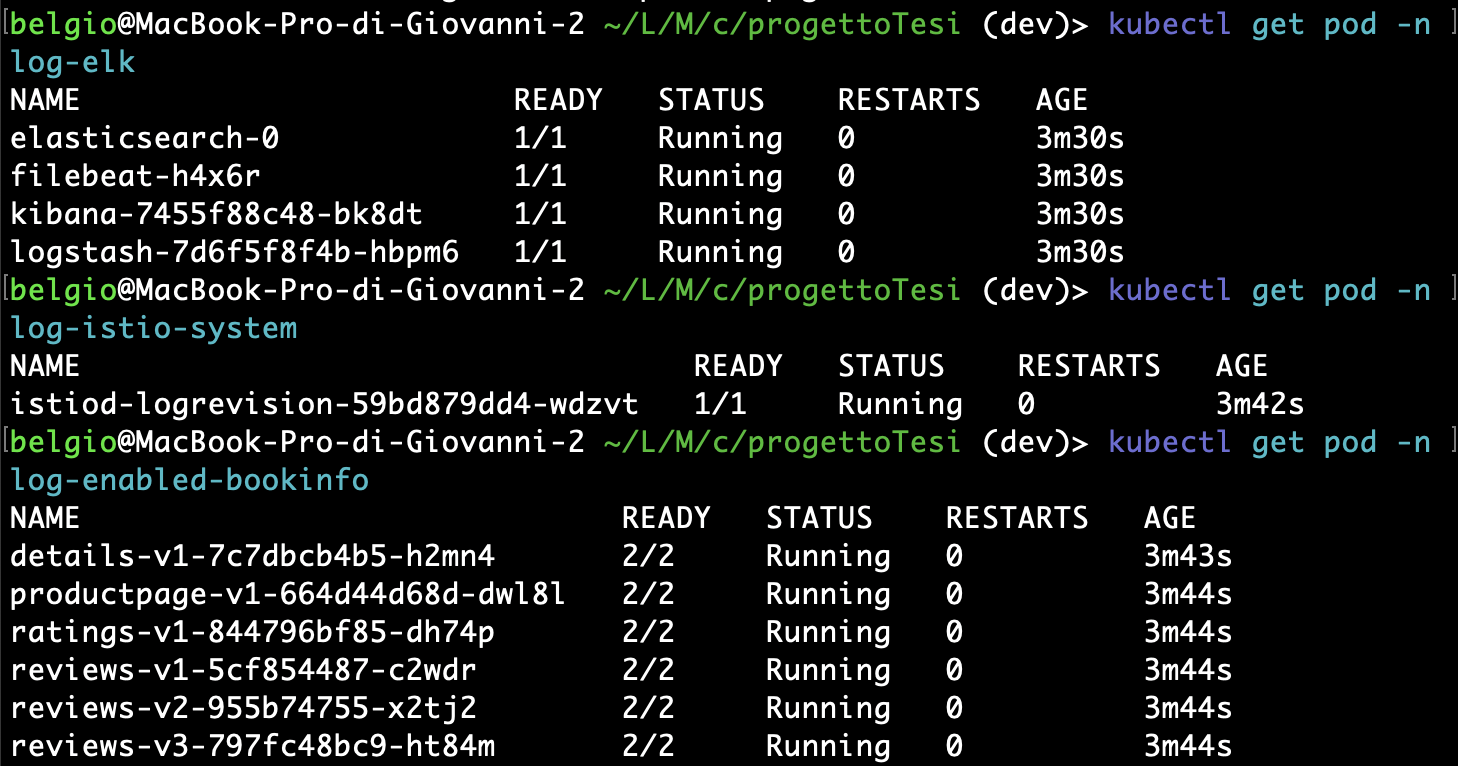
\includegraphics[width=\textwidth]{immagini/capitolo5/kubectl_get_pod.png}
    \caption{Controllo del corretto deploy delle risorse.}
    \label{fig:kubectl_get_pod}
\end{figure}

Tramite Minikube, è possibile esporre dei servizi presenti l'ambiente Kubernetes al sistema host. In particolare, il servizio interessato in questo caso è il servizio \texttt{productpage}, che consente di verificare il corretto funzionamento dello stack di servizi. Ciò è possibile tramite il comando \ref{lst:code_minikube_productpage}:
\begin{lstlisting}[caption={Esposizione del servizio \texttt{productpage} al sistema host.}, label=lst:code_minikube_productpage, language=bash]
minikube service productpage --url -n log-enabled-bookinfo
\end{lstlisting}
Come si osserva in Figura \ref{fig:working}, sia le \texttt{Reviews} che i \texttt{Ratings} vengono serviti correttamente a \texttt{Productpage}.

\begin{figure}[h]
    \centering
    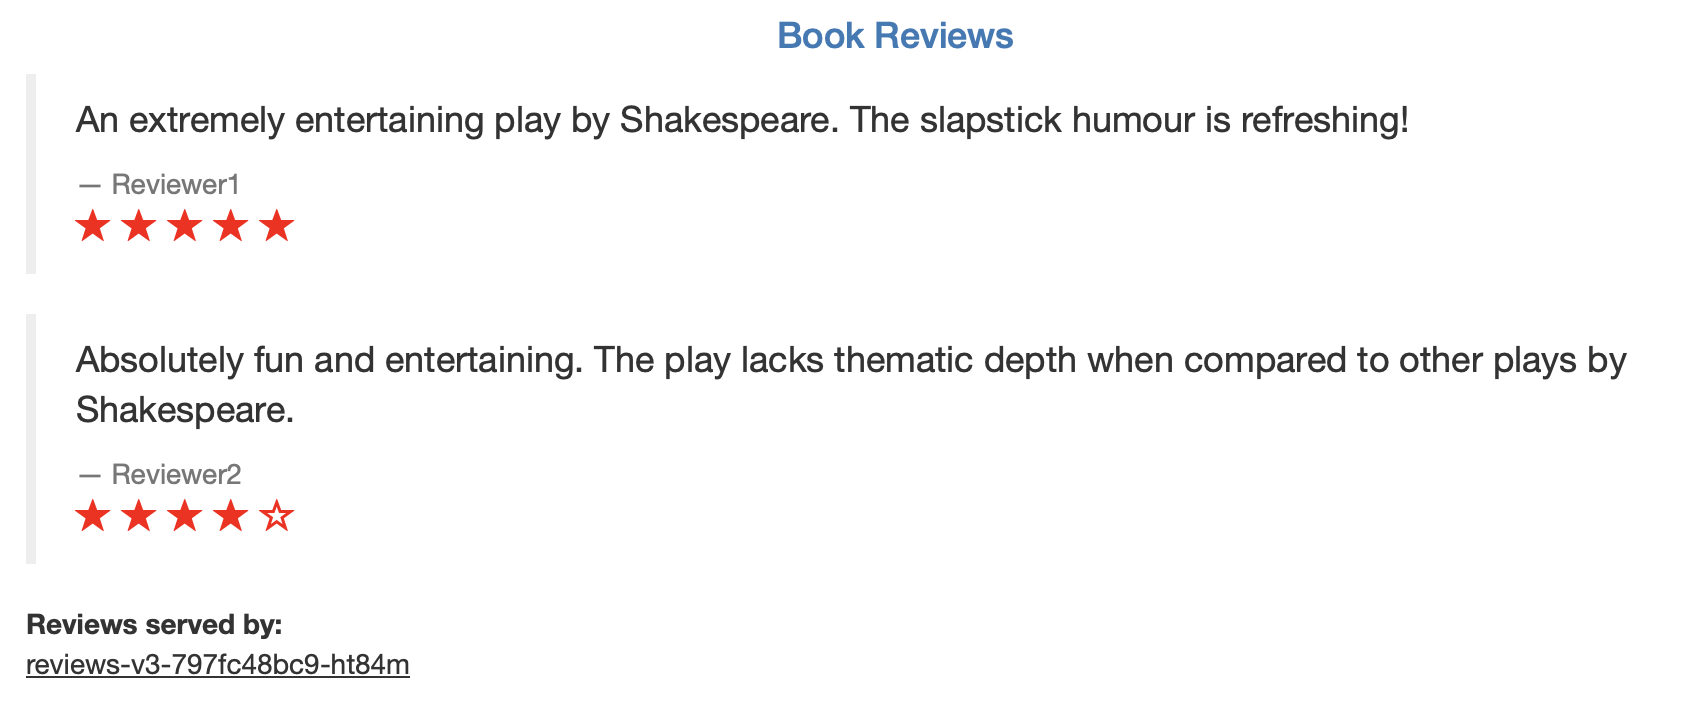
\includegraphics[width=\textwidth]{immagini/capitolo5/working.png}
    \caption{Controllo del funzionamento di \texttt{Productpage}.}
    \label{fig:working}
\end{figure}


Kubectl non mette a disposizione un comando per interrompere l'esecuzione di un fallimento, ma dato che l'ambiente di test è Minikube in esecuzione su Docker, è possibile configurare la shell locale per utilizzare il demone Docker che si trova all'interno di Minikube. Per eseguire ciò, è necessario eseguire il comando \ref{lst:shell_minikube}:

\begin{lstlisting}[caption={Passaggio al demone Docker in Minikube.}, label=lst:shell_minikube, language=bash]
eval $(minikube docker-env)
\end{lstlisting}

Utilizzando il demone Docker all'interno di Minikube, è possibile mettere in pausa l'esecuzione del container, simulando quindi un fallimento interno. Per fare ciò, è necessario eseguire il comando presente nel Codice \ref{lst:grep_ratings}: 
\begin{lstlisting}[caption={Ottenimento del container relativo ai Ratings.}, label=lst:grep_ratings, language=bash]
docker ps | grep k8s\_ratings
\end{lstlisting}

Tramite il comando del Codice \ref{lst:grep_ratings}, è possibile scoprire qual è l'ID del container di \verb|Ratings|, per poi metterlo in pausa. Nell'esempio della Figura \ref{fig:pause}, l'ID associato al container è \texttt{aa42b22e1568}.

A questo punto, è possibile interrompere temporaneamente l'esecuzione di \verb|Ratings|, tramite il comando riportato nel Codice \ref{lst:docker_pause}: 
\begin{lstlisting}[caption={Pausa del container.}, label=lst:docker_pause, language=bash]
docker pause <id_container>
\end{lstlisting}

\begin{figure}[h]
    \centering
    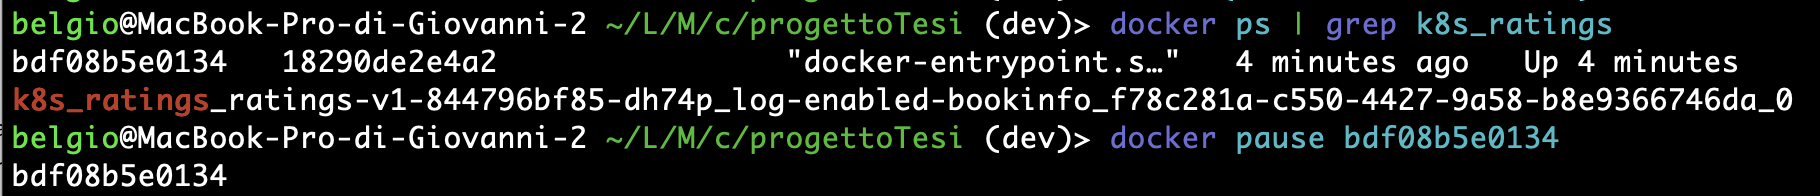
\includegraphics[width=\textwidth]{immagini/capitolo5/pause_cont.png}
    \caption{Container sospeso correttamente.}
    \label{fig:pause}
\end{figure}


Con il container in pausa, il proxy Envoy genererà una stringa di errore, che sarà poi elaborata dallo script Python per produrre l'errore in uno dei formati richiesti. È poi possibile scaricare i log richiesti dall'istanza ElasticSearch eseguendo il comando:
\begin{lstlisting}[caption={Comando per lo scaricamento dei log da ElasticSearch.}, label=lst:log_download, language=bash]
python main.py -c localhost -p <porta> -o <file di output> -n bookinfo
\end{lstlisting}

In Figura \ref{fig:cat_log}, si possono visualizzare parte dei log scaricati in questo test. Visto il lungo messaggio JSON prodotto, in figura viene evidenziata solo la parte \textit{event}:

\begin{figure}[h]
    \centering
    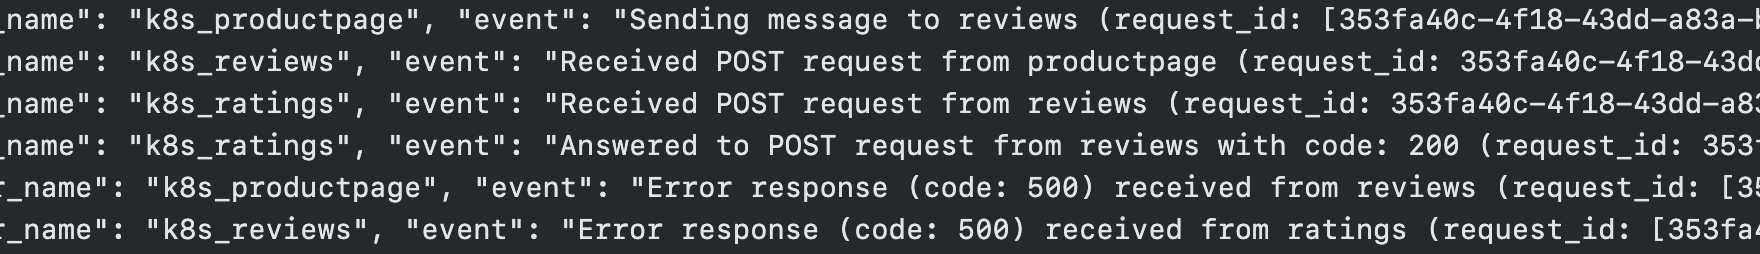
\includegraphics[width=\textwidth]{immagini/capitolo5/cat_log.png}
    \caption{Visualizzazione dei log.}
    \label{fig:cat_log}
\end{figure}

Per provare poi il corretto funzionamento del sistema, è possibile eseguire yRCA per individuare quale sia stata la causa o il motivo del fallimento: infatti, in questo caso, interrogando yRCA sul perché ci sia stato un fallimento, viene correttamente identificato da yRCA che si è trattato del container \texttt{Ratings}, non più operativo.
\begin{figure}[h]
    \centering
    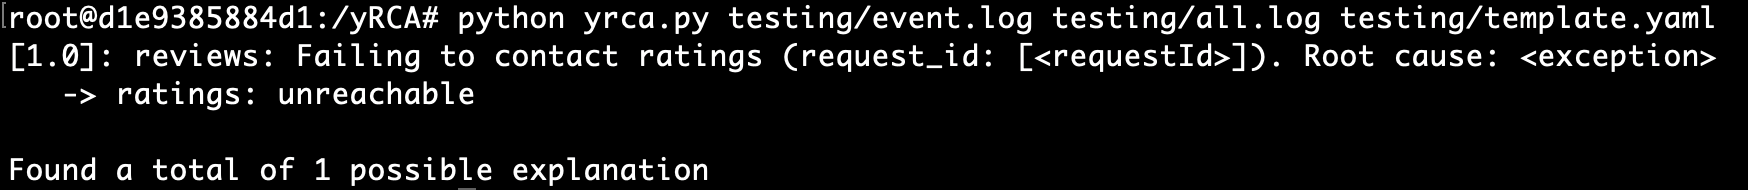
\includegraphics[width=\textwidth]{immagini/capitolo5/bookinfo_yrca.png}
    \caption{Esecuzione di yRCA per spiegare il motivo del fallimento.}
    \label{fig:yrca-error}
\end{figure}


\section{Simulazione di un fallimento con l'applicazione Chaos Echo}
\subsection{Introduzione a Chaos Echo}
Chaos Echo\footnote{https://github.com/di-unipi-socc/chaos-echo} è un'applicazione progettata per testare la resilienza ai fallimenti di un'applicazione a microservizi. Il suo funzionamento è basato sulla ricezione di richieste da parte di un'applicazione esterna, e sulla successiva risposta in maniera aleatoria: o fornendo una risposta entro un certo intervallo di tempo, o inducendo un timeout, simulando così una potenziale interruzione del servizio.

Chaos Echo permette la configurazione dei parametri interni tramite le seguenti variabili d'ambiente:
\begin{itemize}
    \item \texttt{DEPENDS\_ON}: Parametro che indica dei nomi di host che il servizio può a sua volta contattare.
    \item \texttt{TIMEOUT}: Parametro che indica il tempo di timeout, in millisecondi, con il quale si deve attendere una risposta da un servizio contattato.
    \item \texttt{P\_INVOKE}: Parametro con range da 0 a 100, con il quale si indica la probabilità in percentuale che il suddetto servizio chiami a sua volta uno dei servizi specificati nel campo \texttt{DEPENDS\_ON}.
    \item \texttt{P\_FAIL}: Parametro con range da 0 a 100, con il quale si indica la probabilità in percentuale che il servizio non risponda a richieste provenienti da altri servizi o dall'esterno.
    \item \texttt{P\_CRASH}: Parametro con range da 0 a 100, con il quale si indica la probabilità in percentuale che il servizio termini al momento di ricezione della richiesta.
\end{itemize}


In questa seconda casistica di fallimento, l'obiettivo è ancora quello di simulare un fallimento interno, ma differentemente da quanto accaduto nella prima casistica di testing, dove un blocco completo del container impediva sia la ricezione che la trasmissione di richieste e risposte, questa seconda casistica si concentra sullo sviluppare un messaggio di timeout, dove la richiesta viene ricevuta correttamente dal container, ma non viene mai elaborata una risposta, generando un timeout.

\subsection{Iniezione del fallimento}

In questa implementazione, vengono dispiegate tre istanze di Chaos Echo, ognuna con parametri di configurazione differenti:
\begin{itemize}
    \item \textit{Frontend}: \texttt{P\_INVOKE} = 100\%, \texttt{P\_FAIL} = 50\%, \texttt{P\_CRASH} = 0\%, 
    \item \textit{Middle}: \texttt{P\_INVOKE} = 100\%, \texttt{P\_FAIL} = 90\%, \texttt{P\_CRASH} = 0\%, 
    \item \textit{Backend}: \texttt{P\_INVOKE} = 0\%, \texttt{P\_FAIL} = 90\%, \texttt{P\_CRASH} = 70\%, 
\end{itemize}

Quando una chiamata HTTP parte da \textit{curl} e arriva a \textit{frontend}, quest'ultimo la redirige verso \textit{middle}, con le probabilità specificate sopra. Una volta arrivata a \textit{middle}, viene poi indirizzata verso \textit{backend}, che decide se fallire esso stesso, oppure inviare un messaggio di errore.

Per generare le chiamate, è stato creato un file di deployment Kubernetes che unisce le istanze di Chaos Echo con un container che esegue l'immagine \texttt{radial/busyboxplus:curl}\footnote{https://hub.docker.com/r/radial/busyboxplus}. L'unico scopo di quest'ultimo container è eseguire il comando \textit{curl}, e di attendere un tempo predefinito tra una chiamata e l'altra, in modo da simulare le chiamate provenienti da un eventuale servizio esterno.
Il comando utilizzato per tale scopo è:
\begin{lstlisting}
    curl -X POST -H 'Content-Type: application/json' -H 'Cache-Control: no-cache' -i http://$A/echo --data '{ "content": "FRONTEND REQUEST", "hash": "1" }' --silent & 
\end{lstlisting}
Per l'iniezione del fallimento i passi necessari per il dispiegamento del deployment sono identici a quanto descritto per Bookinfo, ma utilizzando Chaos Echo come deployment target. Come richiesto dalla specifica del test, il container con curl inizia a inviare richieste alle istanze di Chaos Echo, e provoca fallimenti di tipo timeout quando la richiesta non viene risposta entro un tempo limite. In questo test, il tempo massimo consentito per l'invio di una risposta prima della generazione dell'errore di timeout è stato fissato ad 1 secondo. In Figura \ref{fig:chaosecho-logs}, sono riportati i messaggi di errore estratti dai log.

\begin{figure}[h]
    \centering
    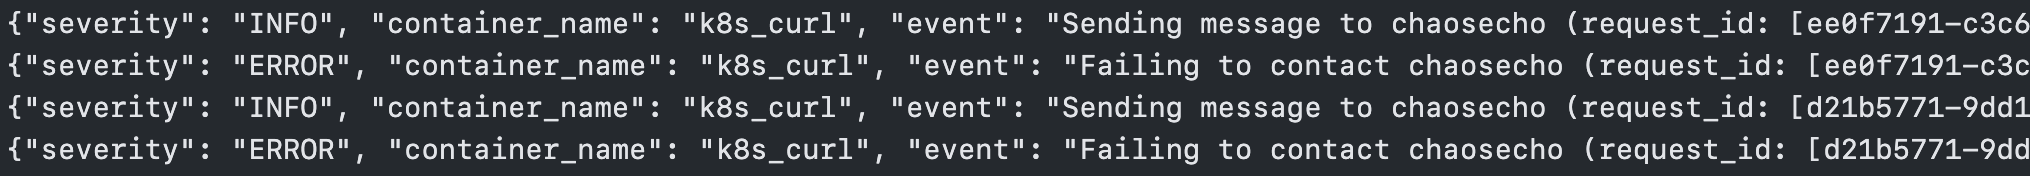
\includegraphics[width=\textwidth]{immagini/capitolo5/chaosecho_logs.png}
    \caption{Visualizzazione dei log.}
    \label{fig:chaosecho-logs}
\end{figure}

Eseguendo il deployment attraverso yRCA, e chiedendo di analizzare l'errore rilevato su \textit{curl}, si può notare quale sia stato il pod che ha causato il fallimento. Infatti, oltre ad essere presente l'errore \myenquote{\texttt{Error response (code: [Response Code]) received from...}}, il messaggio di output è composto da più linee, in quanto l'errore si è propagato \myenquote{a catena} fino ad arrivare a \textit{curl}. yRCA riesce quindi correttamente a ricostruire le interazioni, e a mostrare che a fallire è stato il pod \textit{backend}, in quanto l'ultimo messaggio che è stato inviato da \textit{middle} a \textit{backend} non ha ricevuto risposta, generando un errore di tipo  \myenquote{\texttt{Failing to contact [Service Name]]}}.


\begin{figure}[h]
    \centering
    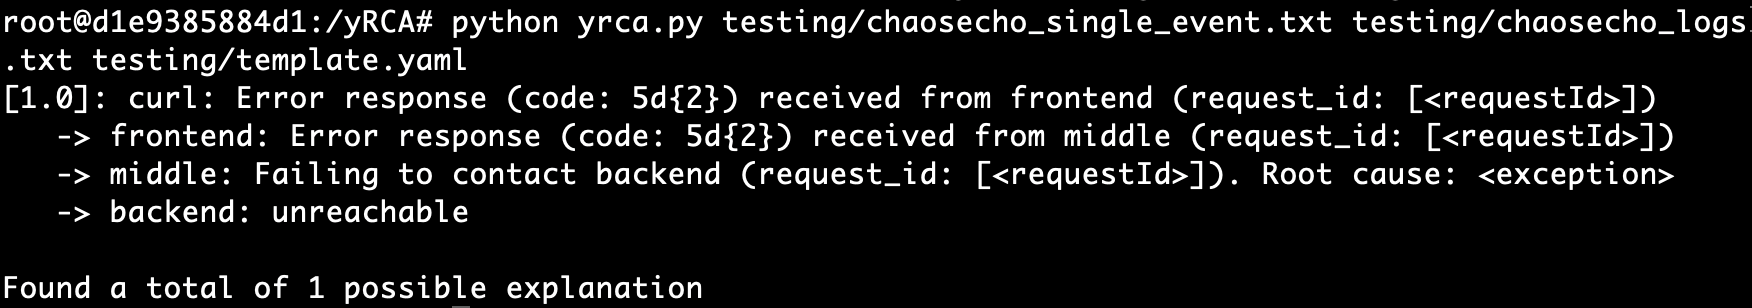
\includegraphics[width=\textwidth]{immagini/capitolo5/chaosecho_yrca.png}
    \caption{Visualizzazione dell'errore.}
    \label{fig:chaosecho-error}
\end{figure}

\section{Iniezione di un fallimento nell'applicazione Online Boutique} \label{sect:Iniezione di un fallimento nell'applicazione Online Boutique}

\subsection{Introduzione a Online Boutique}

Allo stesso modo di Istio con l'applicazione Bookinfo, altre piattaforme offrono applicazioni di esempio per aiutare gli sviluppatori. Una di queste applicazioni è \myenquote{Online Boutique}\footnote{https://github.com/GoogleCloudPlatform/microservices-demo} (o precedentemente conosciuta come \myenquote{Microservices Demo}), che rappresenta un moderno negozio online, funzionante tramite architettura a microservizi.

L'applicazione Online Boutique è composta da una serie di microservizi, tra cui:

\begin{itemize}
    \item \textit{Frontend:} Il front-end dell'applicazione, responsabile dell'interfaccia utente.
    \item \textit{Cart-service:} Gestisce il carrello della spesa dell'utente.
    \item \textit{Checkout-service:} Si occupa del processo di pagamento.
    \item \textit{Product-catalog-service:} Contiene il catalogo dei prodotti disponibili.
    \item \textit{Shipping-service:} Calcola i costi di spedizione.
    \item \textit{Payment-service:} Gestisce le transazioni di pagamento.
\end{itemize}

Per questo test, si vuole simulare un fallimento nel microservizio \textit{Payment-service}. Infatti, un fallimento in questo punto, non permette mai all'utente di completare l'acquisto, indipendentemente da quale articolo si vada ad acquistare. In particolare, si vuole creare un fallimento di tipo \myenquote{never started}, che si verifica quando il microservizio fallisce prima di generare log.

\subsection{Iniezione del fallimento}

Dopo aver eseguito lo script Python per modificare il deployment, ed averlo dispiegato correttamente nel cluster seguendo i passaggi illustrati per Bookinfo, si può procedere con la simulazione del fallimento simulando un blocco interno al container. Non appena viene creata la risorsa su Kubernetes, viene immediatamente portato a zero il numero di repliche del deployment \textit{payment-service}, per impedire ad esso di generare log. Ciò viene svolto tramite il comando presente nel Codice \ref{lst:paymentservice_zero}:
\begin{lstlisting}[caption={Configurazione del numero di repliche di \textit{payment-service.}}, label=lst:paymentservice_zero, language=bash]
    kubectl scale deployment paymentservice --replicas=0
\end{lstlisting}

Una volta generati i log con i metodi descritti al Capitolo \ref{sect:Iniezione di un fallimento nell'applicazione Bookinfo}, è possibile eseguire yRCA per ottenere il servizio che ha causato la serie di fallimenti a catena. Si chiede quindi a yRCA di ispezionare il log di errore del pod \textit{checkout-service}, essendo il pod che gestisce tutto il processo di acquisto \textit{(Figura \ref{fig:paymentservice_unreachable})}.

\begin{figure}[h]
    \centering
    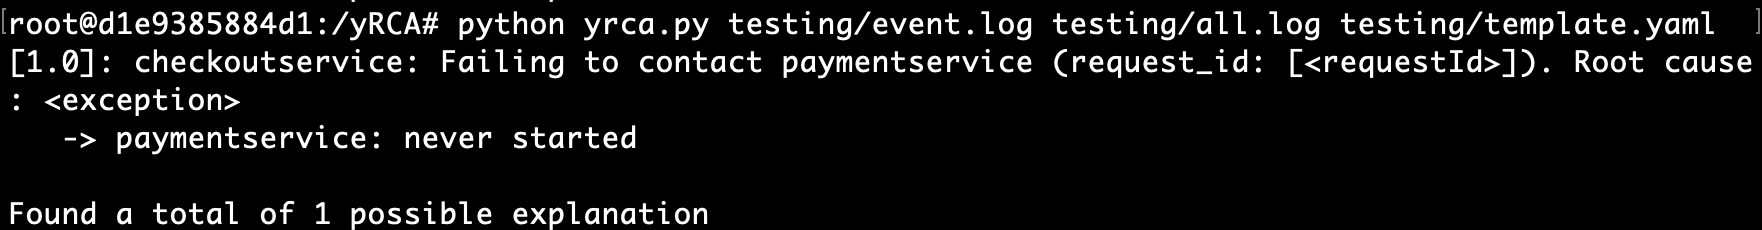
\includegraphics[width=\textwidth]{immagini/capitolo5/paymentservice_neverstarted.png}
    \caption{Analisi della causa di fallimento nell'applicazione Online Boutique.}
    \label{fig:paymentservice_unreachable}
\end{figure}

Dopo l'elaborazione, yRCA riporta correttamente la causa di errore, scoprendo che il pod a fallire è stato \textit{payment-service}, e che esso probabilmente non fosse mai stato avviato, non avendo mai generato log prima del fallimento.


\section{Iniezione di un fallimento nell'applicazione Sock Shop}

\subsection{Introduzione a Sock Shop}
Sock Shop\footnote{https://github.com/microservices-demo/microservices-demo} è un'applicazione demo a microservizi progettata per dimostrare il paradigma a microservizi in un e-commerce. Si tratta di un negozio online dove gli utenti possono visualizzare, cercare e acquistare calzini. L'applicazione utilizza diversi linguaggi e tecnologie per mostrare un approccio poli-tecnologico ai microservizi. 

L'architettura di Sock Shop comprende vari componenti, tra cui:

\begin{itemize}
    \item \textit{Front-End:} Interfaccia utente web del negozio.
    \item \textit{Catalogue:} Microservizio che gestisce l'inventario dei calzini disponibili.
    \item \textit{Cart:} Gestisce il carrello della spesa dell'utente.
    \item \textit{User:} Gestione degli utenti e delle sessioni di accesso.
    \item \textit{Orders:} Microservizio che gestisce gli ordini degli utenti.
    \item \textit{Shipping:} Si occupa delle spedizioni.
    \item \textit{Payment:} Gestione delle transazioni di pagamento.
\end{itemize}

Molti microservizi di questa applicazione hanno un database associato, che memorizza le informazioni persistenti relative alle funzionalità del microservizio. Ad esempio, il microservizio \myenquote{Catalogue} avrà un database che memorizza tutti i dettagli sui calzini disponibili, come nome, descrizione, prezzo e immagine. È possibile riconoscere ogni database dal microservizio associato, in quanto presenta una nomenclatura uguale a quest'ultimo, ma con il suffisso \texttt{-db}.

In Figura \ref{fig:sockshop-graph}, è osservabile un grafo dell'applicazione Sock Shop.

\begin{figure}[h]
    \centering
    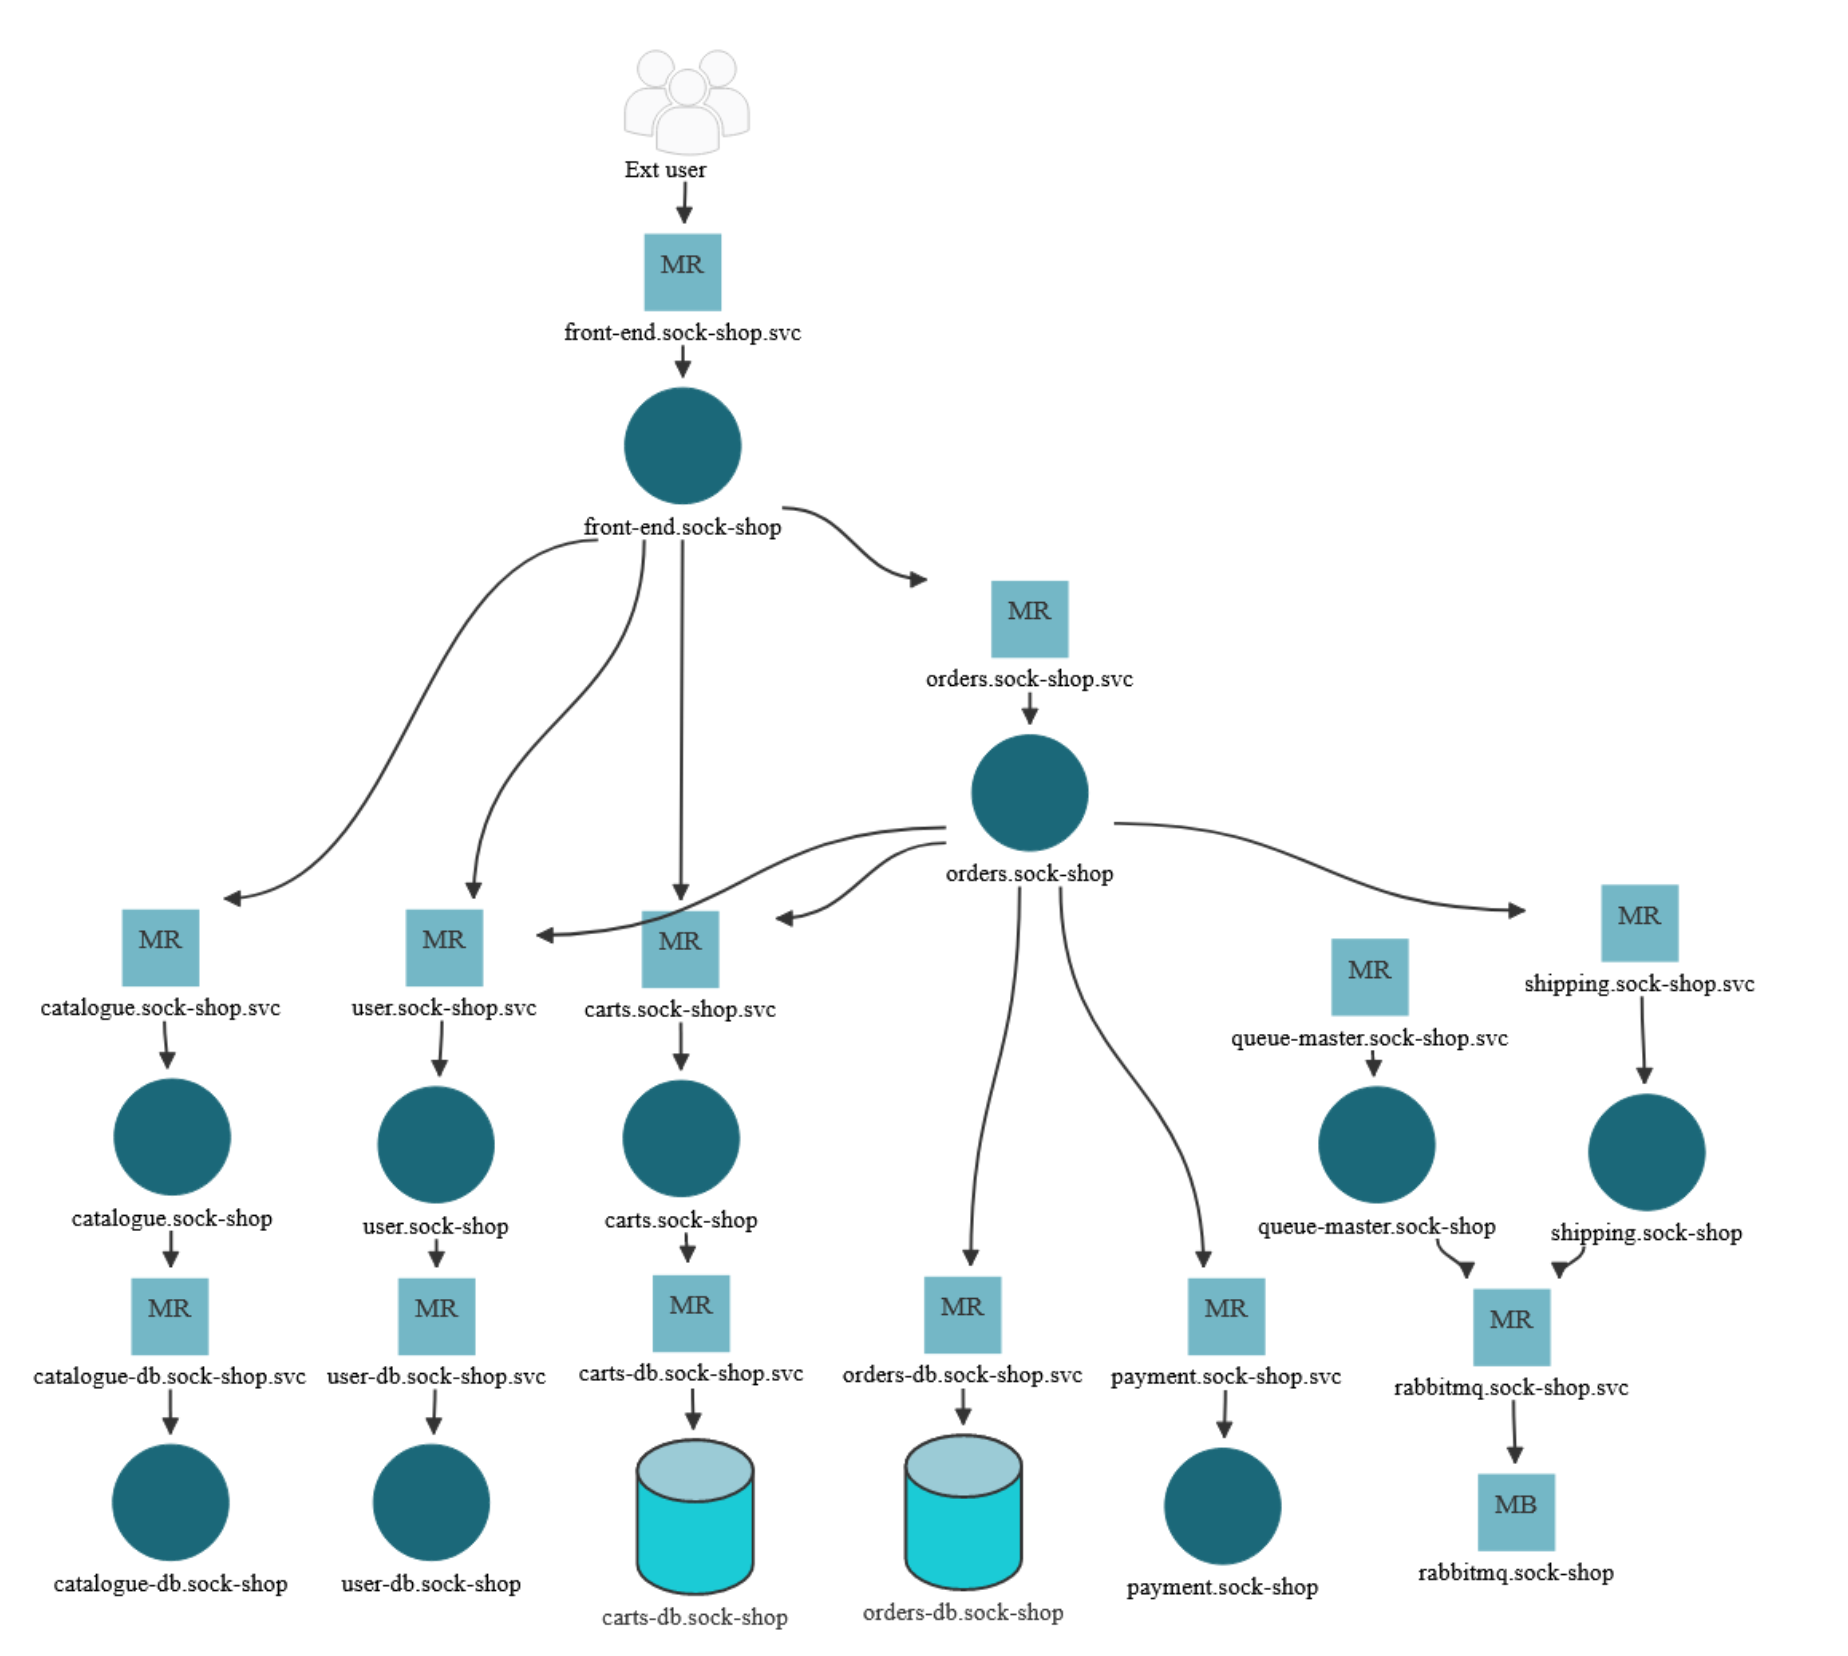
\includegraphics[width=\textwidth]{immagini/capitolo5/sockshop_graph.png}
    \caption{Grafo dell'applicazione a microservizi Sock Shop \cite{sockshop_graph}.}
    \label{fig:sockshop-graph}
\end{figure}

\subsection{Iniezione del fallimento}
Per testare il sistema con Sock Shop, verrà simulato un fallimento nel servizio \texttt{carts}. Il fallimento di questo componente rende impossibile l'aggiunta e la rimozione degli elementi dal carrello.

Anche in questo test, la preparazione dell'ambiente relativa al dispiegamento del deployment di Sock Shop modificato è identica a quella vista per gli altri test. Dopo aver sospeso l'esecuzione di \texttt{carts}, il sito è rimasto ancora completamente visitabile e navigabile, ma aggiungere prodotti al carrello non sembrava avere effetto dall'interfaccia browser, e ispezionando l'errore utilizzando la console di sviluppo del browser, è stato possibile notare l'errore riportato in Figura \ref{fig:sockshop-error}.

\begin{figure}[h]
    \centering
    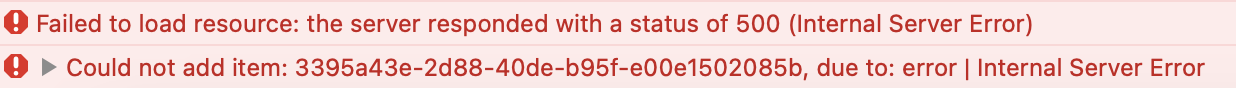
\includegraphics[width=\textwidth]{immagini/capitolo5/browser_error.png}
    \caption{Errore nella console browser.}
    \label{fig:sockshop-error}
\end{figure}

Come effettuato per i test precedenti, è stato possibile analizzare il fallimento con yRCA, consentendo quindi di scoprire quale sia stato il pod a causare i fallimenti \textit{(Figura \ref{fig:sockshop-yrca})}.

\begin{figure}[h]
    \centering
    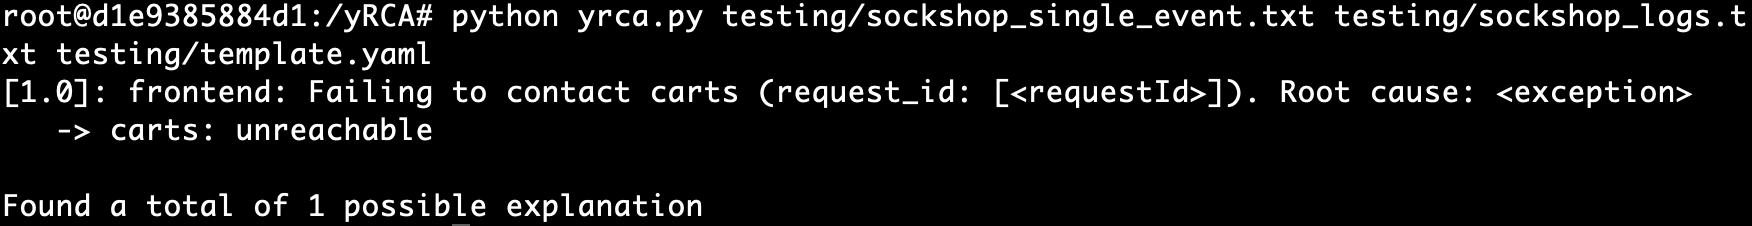
\includegraphics[width=\textwidth]{immagini/capitolo5/new_sockshop_yrca.png}
    \caption{Spiegazione del fallimento nell'applicazione Sock Shop.}
    \label{fig:sockshop-yrca}
\end{figure}

\section{Analisi delle prestazioni}
\subsection{Introduzione}
Un aspetto importante relativo alla validazione della soluzione è analizzare che la stessa abbia sul cluster un impatto prestazionale accettabile e generalmente proporzionato alla complessità dell'ambiente che si vuole monitorare. È infatti necessario che la soluzione proposta non introduca un \textit{overhead}, tale da far sì che i benefici derivati dall'implementazione della soluzione proposta non siano giustificati dal costo che la stessa soluzione ha in termini di risorse.

Per l'analisi delle prestazioni, sono state considerate le seguenti metriche:

\begin{itemize}
    \item \textbf{Utilizzo CPU e RAM:} metriche per misurare l'overhead della soluzione in termini di utilizzo di CPU e memoria RAM. È importante notare che su Kubernetes l'unità di misura per il consumo della CPU è il \myenquote{core}, che rappresenta un'unità logica del processore. Questo valore indica quanta capacità di elaborazione CPU un'applicazione o servizio sta utilizzando all'interno di un pod.
    \item \textbf{Utilizzo delle immagini:} metrica che misura lo spazio occupato da tutte immagini Docker dai componenti della soluzione.
    \item \textbf{Tempi di latenza:} metrica per misurare la variazione del tempo di risposta di un'applicazione a microservizi quando la soluzione viene applicata. 

\end{itemize}

Tutti i test sono stati svolti su Minikube in esecuzione su un ambiente Docker, con 8 GB di RAM e 8 threads CPU dedicati.

\subsection{Analisi di CPU e RAM}
Per lo scopo di questo test, sono stati posti sotto test tre dei quattro dispiegamenti trattati nel Capitolo \ref{chap:Validazione della soluzione}. È stato infatti deciso di analizzare l'utilizzo CPU e RAM nei deployment di applicazioni realistiche, ovvero:
\begin{itemize}
    \item \textit{Online Boutique}
    \item \textit{Bookinfo}
    \item \textit{Sock Shop}
\end{itemize}

Per monitorare l'utilizzo di CPU e RAM della soluzione, è necessario in primis installare il \textit{Metrics Server}\footnote{https://github.com/kubernetes-sigs/metrics-server}, un componente che consente di ottenere i dati relativi alle metriche sulle prestazioni dai Kubelet, per poi esporle all'API Server tramite le \textit{Metrics API}. Quest'ultime sono poi accessibili tramite il comando presente nel Codice \ref{lst:kubectl-metrics}:
\begin{lstlisting}[caption={Comando per la rilevazione di metriche.}, label=lst:kubectl-metrics, language=bash]
    kubectl top pods -n <nome del namespace da monitorare>
\end{lstlisting}

Per ottenere una percentuale di overhead, è necessario ottenere il consumo di CPU e RAM per un dispiegamento con funzionalità di raccolta del logging, e compararlo allo stesso deployment, ma senza le suddette funzionalità abilitate.

Nella Tabella \ref{table:cpu_analysis}, è possibile notare l'utilizzo di CPU e RAM del dispiegamento Online Boutique, con le funzioni di logging abilitate. Tali metriche sono state rilevate più volte, nell'arco di 5 minuti, mentre verso il cluster viaggiava un traffico costante di richieste GET. I valori non si sono mai discostati in modo significativo da quelli riportati in Tabella \ref{table:cpu_analysis}.

\begin{table}[h]
\centering
\begin{tabular}{|l|l|c|c|c|}
\hline
\rowcolor{lightgray}
\textbf{Applicazione} & \textbf{Tipo} & \textbf{CPU (m)} & \textbf{RAM (MB)} & \textbf{Overhead \%} \\
\hline
\multirow{2}{*}{Online-Boutique} & Base & 181m & 586 MB & \multirow{2}{*}{CPU: 131.49\%, RAM: 646.42\%} \\
& Con logging & 419m & 4374 MB & \\
\hline
\multirow{2}{*}{Bookinfo} & Base & 197m & 760 MB & \multirow{2}{*}{CPU: 170.56\%, RAM: 441.32\%} \\
& Con logging & 533m & 4114 MB & \\
\hline
\multirow{2}{*}{Sock Shop} & Base & 161m & 2825 MB & \multirow{2}{*}{CPU: 463.35\%, RAM: 128.96\%} \\
& Con logging & 907m & 6468 MB & \\
\hline
\end{tabular}
\caption{Confronto dell'utilizzo delle risorse per i tipi di dispiegamento.}
\label{table:cpu_analysis}
\end{table}

Per il dispiegamento Online Boutique, si dà in Figura \ref{fig:perf_analysis} anche un dettaglio dell'utilizzo CPU e RAM tra i pod dei vari namespace.

\begin{figure}[h]
    \centering
    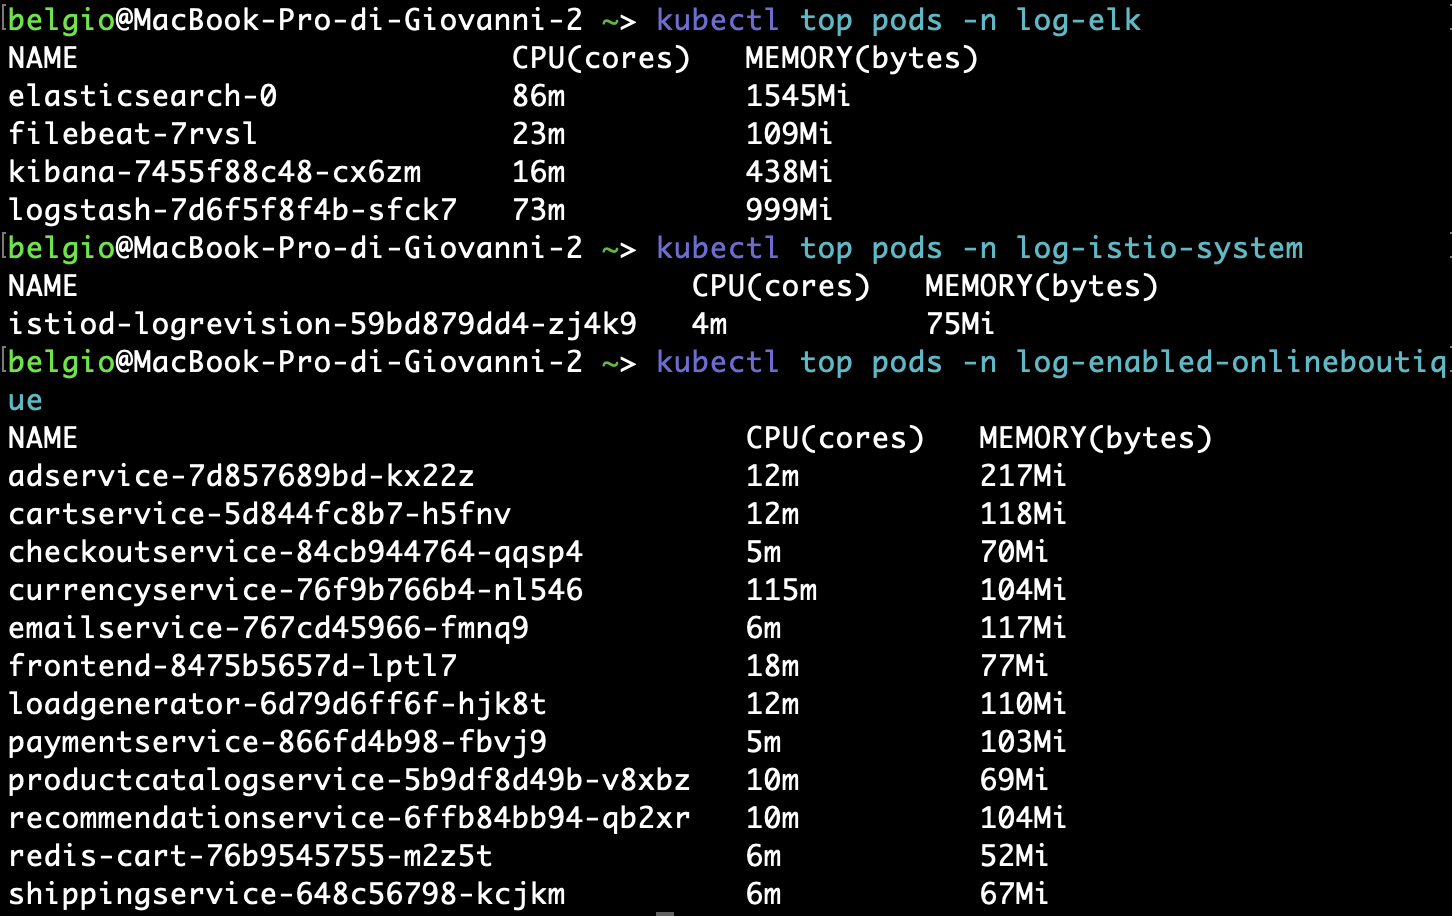
\includegraphics[width=\textwidth]{immagini/capitolo5/cpu_onlineboutique.png}
    \caption{Visualizzazione del consumo di CPU e RAM dei singoli componenti per il dispiegamento Online Boutique.}
    \label{fig:perf_analysis}
\end{figure}

\subsection{Analisi dell'utilizzo di storage delle immagini}
Per procedere all'analisi delle metriche sull'utilizzo dello storage, viene usato il supporto Docker integrato a Minikube, descritto nel Capitolo \ref{Iniezione del fallimento}. Una volta attivato, è possibile tramite vedere l'utilizzo di tutte le immagini presenti nel cluster tramite il comando:
\begin{lstlisting}
    docker images
\end{lstlisting}
Per questo test, i dati riportati per lo storage sono presenti nella Tabella \ref{tab:storage_usage}.
\begin{table}[H]
    \centering
    \begin{tabular}{|c|c|}
    \hline
    \rowcolor{lightgray}
        Nome immagine & Utilizzo \\ \hline
       Istiod  &  167 MB \\ \hline
       Proxy Envoy & 241 MB\\ \hline
       ElasticSearch  & 837 MB\\ \hline
       Logstash & 1,68 GB\\ \hline
       Kibana & 1,27 GB\\ \hline
       Filebeat & 1,16 GB\\ \hline
      \rowcolor{lightgray}
      Totale & 5,35 GB \\ \hline
    \end{tabular}
    \caption{Tabella sull'utilizzo dell'archiviazione.}
    \label{tab:storage_usage}
\end{table}
Come è possibile rilevare, la maggior parte dell'archiviazione è occupata dai componenti dello stack ELK, in quanto trattasi di servizi complessi, con un grande numero di funzionalità, e che necessitano di svariate dipendenze e librerie. Al contrario, è stato rilevato che Istio e i Proxy Envoy utilizzano una quantità molto minore di archiviazione, con una somma che arriva a 408 MB di spazio utilizzato.

La Tabella \ref{table:storage_comparison} mostra invece quanto vadano ad incidere, in termini  assoluti e percentuali, le componenti di Istio e dello stack ELK sullo spazio di archiviazione complessivo per ciascuna applicazione.

\begin{table}[h]
\centering
\begin{tabular}{|l|c|c|c|}
\hline
\rowcolor{lightgray}
\textbf{Applicazione} & \textbf{Base} & \textbf{Con logging} & \textbf{Overhead (\%)} \\
\hline
Bookinfo & 2377 MB & 7732 MB & 225.28 \% \\
\hline
Online Boutique & 1712,2 MB & 7067,2 MB & 312,76 \% \\
\hline
Sock Shop & 2991,4 MB & 8346,4 MB & 179,01 \% \\
\hline
\end{tabular}
\caption{Overhead per l'archiviazione nelle varie applicazioni di test.}
\label{table:storage_comparison}
\end{table}




\subsection{Analisi della latenza}
L'ultima metrica oggetto di analisi è stata la latenza. In particolare, si è voluto analizzare quanto la soluzione proposta impattasse i tempi delle interazioni tra i pod del cluster. A differenza delle metriche misurate nei capitoli precedenti, dove l'overhead è direttamente proporzionale al numero di container o risorse utilizzate, l'overhead per i tempi di latenza dipende maggiormente dal numero di interazioni scambiate tra i pod. La causa di questo overhead è potenzialmente attribuibile al proxy Envoy, che agendo da componente che intercetta ogni chiamata tra i pod, introduce un quantitativo di latenza in ogni comunicazione. Per comprendere se ciò potesse impattare in modo significativo, è stato fondamentale analizzare e confrontare la latenza tra le richieste effettuate in un ambiente con e senza la soluzione proposta. È stato quindi sviluppato uno script \textit{Bash} in grado di eseguire i test oggetto di analisi. Tale script si avvale dello strumento di benchmarking \texttt{wrk}\footnote{https://github.com/wg/wrk} per generare carichi di lavoro e misurare la latenza delle richieste HTTP. Le sperimentazioni sono state condotte simulando diversi scenari d'uso, variando il numero di connessioni contemporanee (per simulare un numero variabile di potenziali utenti), e dispiegando i componenti singolarmente, per misurare l'impatto di ognuno sul sistema. 
In particolare, i test sono stati effettuati con:
\begin{itemize}
    \item \textbf{Deployment base:} Il dispiegamento originale, senza la soluzione applicata.
    \item \textbf{Deployment con Istio:} Il dispiegamento base, con in aggiunta solo i componenti di Istio.
    \item \textbf{Deployment con Istio + ELK:} Il dispiegamento con tutti i componenti della soluzione proposta.
\end{itemize}
Lo script Bash è composto dai seguenti passi:
\begin{enumerate}
    \item \textbf{Applicazione del deployment:} Viene applicato al cluster il deployment di test tramite il comando \texttt{kubectl apply}.
    \item \textbf{Attesa:} Vengono attesi 120 secondi tra l'applicazione delle risorse e l'inizio del testing, in modo da attendere che tutte le risorse siano dispiegate ed avviate correttamente.
    \item \textbf{Test:} Viene eseguito \texttt{wrk}, configurato per essere eseguito più volte, variando tra di loro il numero di connessioni da tenere attive contemporaneamente. In particolare, i test sono stati svolti con 8, 25, 50 e 200 connessioni contemporanee aperte, per simulare più casi d'uso. Tutti i test vengono eseguiti con un tempo limite fissato a 60 secondi.
    \item \textbf{Rimozione del deployment:} Il deployment testato viene rimosso dal cluster, in modo tale da poter eventualmente eseguire nuovamente lo script con un altro deployment senza creare interferenze.
    \item \textbf{Output dei dati:} Lo script restituisce l'output di \texttt{wrk} su un file, il quale nome è specificato come parametro di input.
\end{enumerate}
Come dispiegamento di test, è stato scelto Bookinfo, in quanto trattasi di un'applicazione con una struttura semplice e già trattata nella tesi al Capitolo \ref{sect:Iniezione di un fallimento nell'applicazione Bookinfo}, ma che coinvolge comunque diverse interazioni tra microservizi in una singola chiamata HTTP GET.

Nella Tabella \ref{table:tabella_latenze}, è possibile vedere il risultato dei test effettuati sull'ambiente Bookinfo.


\begin{table}[h]
\centering
\begin{tabular}{|c|c|c|c|c|c|}
\hline
\rowcolor{lightgray}
\textbf{Utenti} & \textbf{Deployment} & \textbf{Latenza AVG} & \textbf{Latenza Stdev} & \textbf{Richieste/sec} & \textbf{Overhead \%} \\
\hline
\multirow{3}{*}{8} & Base & 34.62ms & 28.64ms & 248.26 & - \\
& con Istio & 63.18ms & 37.09ms & 130.31 & 82.5\% \\
& con Istio + ELK & 67.32ms & 40.92ms & 122.92 & 94.4\% \\
\hline
\multirow{3}{*}{25} & Base & 97.70ms & 45.11ms & 252.60 & - \\
& con Istio & 101.06ms & 45.84ms & 243.37 & 3.44 \% \\
& con Istio + ELK & 108.07ms & 28.55ms & 221.85 & 10.6 \% \\
\hline
\multirow{3}{*}{50} & Base & 180.12ms & 24.49ms & 265.55 & - \\
& con Istio & 191.75ms & 22.38ms & 249.79 & 6.5\% \\
& con Istio + ELK & 219.20ms & 35.49ms & 218.59 & 21.7\% \\
\hline
\multirow{3}{*}{200} & Base & 784.47ms & 91.08ms & 253.53 & - \\
& con Istio & 829.61ms & 57.54ms & 239.13 & 5.8\% \\
& con Istio + ELK & 941.63ms & 107.88ms & 210.67 & 20.0\% \\
\hline
\end{tabular}
\caption{Misurazioni rilevate nell'ambiente Bookinfo.}
\label{table:tabella_latenze}
\end{table}




Come è possibile notare, la latenza aumenta proporzionalmente all'aumentare del numero di utenti che interagiscono con l'applicazione. Questo comportamento è atteso, dato che un maggior numero di richieste mette sotto stress il sistema e può portare, come in questo caso, a ritardi nella risposta. Anche la presenza di Istio e ELK influisce sul tempo di risposta, con una latenza che tende ad aumentare in presenza di questi strumenti rispetto al deployment base. Ciò è in linea con quanto atteso, visto che l'introduzione di proxy come Envoy e l'overhead aggiuntivo introdotto dallo stack ELK per la raccolta di log possono anch'essi aggiungere ritardi nelle comunicazioni.

In particolare, si nota che:
\begin{itemize}
\item Con carico pari a 8 utenti, il deployment con Istio presenta una latenza media di circa 30ms in più rispetto al deployment base. Questo test, effettuato unicamente per completezza, non risulta però essere di particolare rilevanza, vista l'alta variabilità dei dati (dato rilevato dalla deviazione standard), che porta ad un'altissima percentuale di overhead. Questa variabilità è probabilmente dovuta al port forwarding che Minikube, in esecuzione su Docker, esegue per rendere disponibili i servizi al sistema host \cite{ibm_report_docker}.
\item Al crescere degli utenti, i dati diventano sempre man mano più consistenti, ed è possibile ottenere delle stime sempre più precise. L'overhead introdotto dallo stack ELK si attesta circa al 20\%, mentre quello relativo ad Istio è di pochi punti percentuale.
\item Sono stati svolti test anche con un numero superiore di connessioni (500 e 1000), ma questi test non hanno riportato nessuna informazione utile, perché l'ingente numero di connessioni ha portato al sovraccarico dell'ambiente di test, risultando nella quasi totalità delle risposte in timeout.
\end{itemize}

È importante menzionare che questi test sono stati eseguiti con l'unico scopo di ottenere un'idea generale dell'incremento di latenza con l'aggiunta della soluzione proposta, ma possono non rispecchiare veri casi d'uso in un cluster. Infatti, i test sono stati condotti in un ambiente Minikube, che rappresenta un ambiente di sviluppo locale e su nodo singolo per Kubernetes. L'hardware, la configurazione e i limiti imposti da Minikube non sono rappresentativi di un vero ambiente di produzione. Pertanto, i risultati ottenuti possono variare significativamente quando la soluzione proposta viene applicata in un vero cluster Kubernetes su un'infrastruttura adeguata.